% /solutions/conference-talks/conference-ornate-20min.fr.tex, 22/02/2006 De Sousa
\documentclass{beamer}
\usepackage{listings}
\usepackage{mdframed}
\usepackage{tikz}
% Ce fichier est un exemple d'expos\'e

% - pour des conf\'erences,
% - d'une dur\'ee approximative de 20 minutes,
% - avec un style ornemental.


% Copyright 2004 by Till Tantau <tantau@users.sourceforge.net>.
%
% Traduction de Philippe De Sousa <philippejjg@free.fr>
%
% En principe, ce fichier peut être redistribu\'e et/ou modifi\'e conform\'ement
% aux termes de la GNU Public License, version 2.
%
% Cependant, ce fichier est suppos\'e comme \'etant un "exemple-type" qui peut être modifi\'e
% selon vos propres besoins. Pour cette raison, si vous utilisez ce fichier en tant qu'
% "exemple-type" et non sp\'ecifiquement pour le distribuer en tant que partie d'un
% package ou programme, je vous donne la permission exceptionnelle de copier librement et
% de modifier ce fichier et même d'effacer ce message de copyright.
\usepackage{pdfpages}

\usepackage[francais]{babel}
% or autre comme par exemple \usepackage[english]{babel}

\usepackage[utf8]{inputenc}
% or autre

\usepackage{float}
\usepackage{graphicx}
\usepackage{wrapfig}
\usepackage{times}
\usepackage[T1]{fontenc}
\makeatletter
\hypersetup{pdfpagemode=FullScreen}

\newcommand{\firstlogo}{images/logos/FACT_official.png}
\newcommand{\secondlogo}{images/logos/ups.jpg}
\newcommand{\footsubject}{Quels sont les systèmes à mettre en œuvre pour offrir une expérience sociale depuis sa télévision ?} % Subject in footer

\newcommand{\rgbcolortheme}{75,106,149}

\mode<presentation> {
\usepackage{../beamer-theme/beamerthemeUNLTheme}
}

\title[] % (facultatif, \`a utiliser uniquement si le titre de l'article est trop long)
{La télévision sociale}
\subtitle{Travail Encadré de Recherche}

\author[
\textbf{F}lorent\\
\textbf{A}ntoine\\
\textbf{C}édric\\
Manan\textbf{T}soa
] % (facultatif, \`a utiliser seulement avec plusieurs auteurs)
{Antoine de \bsc{Roquemaurel}\newline Florent \bsc{Berbie}\newline Cédric \bsc{Rohaut}\newline Manantsoa Andriamihary \bsc{Razanajatovo}}

\institute[] % (facultatif mais g\'en\'eralement n\'ecessaire)
{
  Universit\'e Toulouse III -- Paul Sabatier \\
  M1 Informatique -- Développement Logiciel 
  \vspace{-10px}
}

\date[ ~ ~ ~ 05 / 03 / 2015] % (facultatif, peut être une abr\'eviation du nom de la conf\'erence)
{Vendredi 06 Mars 2015}

\subject{~}

 \pgfdeclareimage[width=2.5cm]{le-logo}{images/logos/FACT_official.png}
 \logo{\pgfuseimage{le-logo}}


% \`a supprimer si vous ne voulez pas que la table des mati\`eres apparaisse
% au d\'ebut de chaque sous-section : 
\AtBeginSection[] {
  \begin{frame}<beamer>{Ligne directrice}
    \tableofcontents[currentsection]
  \end{frame}
}
% Si vous souhaitez recouvrir vos transparents un \`a un,
% utilisez la commande suivante (pour plus d'info, voir la page 74 du manuel
% d'utilisation de Beamer (version 3.06) par Till Tantau) :

%\beamerdefaultoverlayspecification{<+->}


\begin{document}
	\begin{frame}
		\titlepage
	\end{frame}
	\begin{frame}{Introduction}
	\begin{itemize}
		\item Les objets sont de plus en plus connectés\\
			$\Rightarrow$ Internet des objets
		\pause
		\vfill
		\item La télévision est limitée sur le plan social
	\end{itemize}
		\vfill
			\begin{figure}[H]
				\centering
				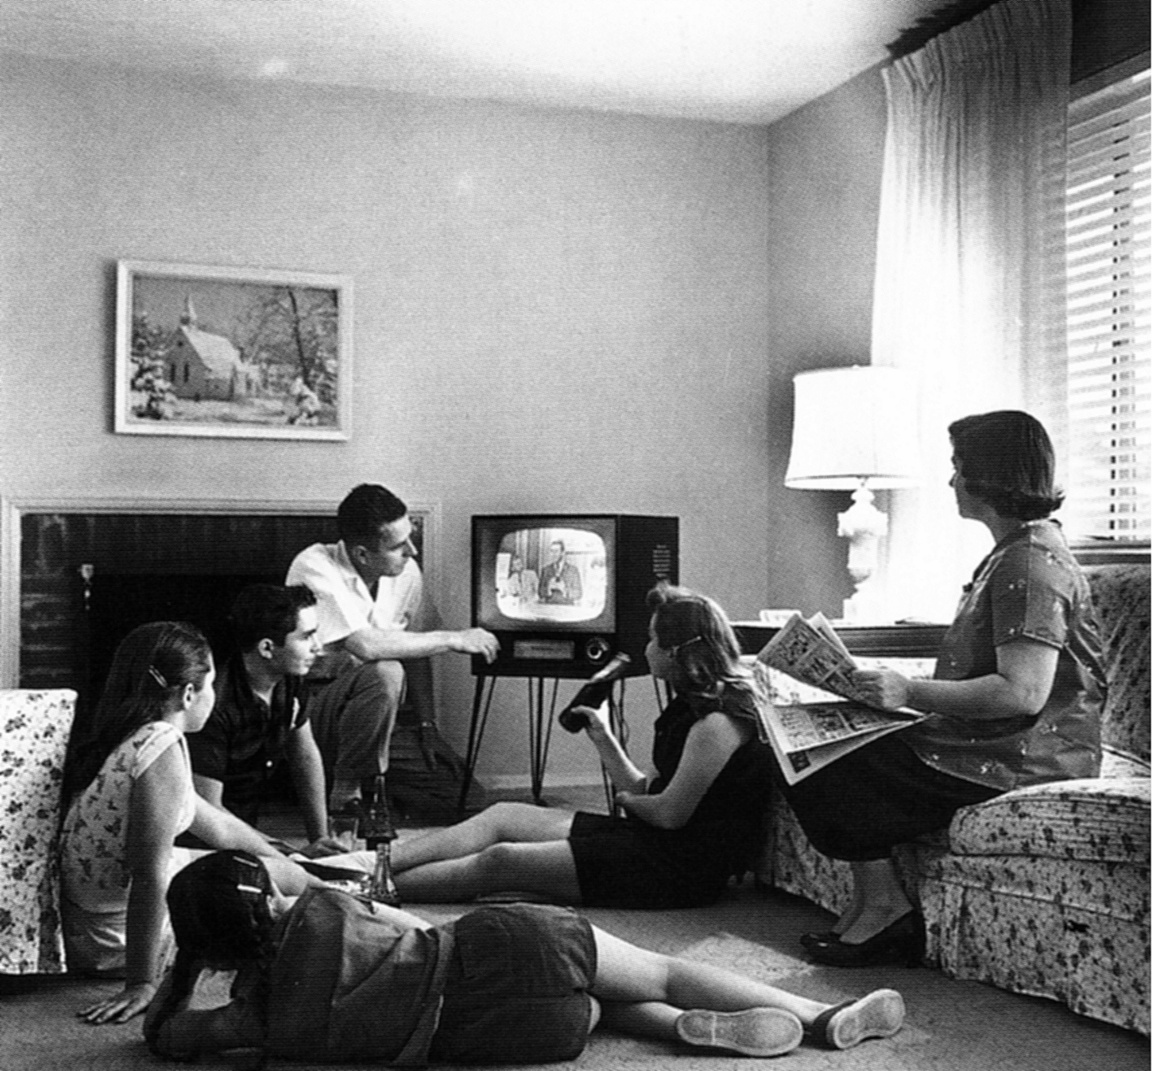
\includegraphics[height=3.4cm]{images/intro/old.jpg}~~~
				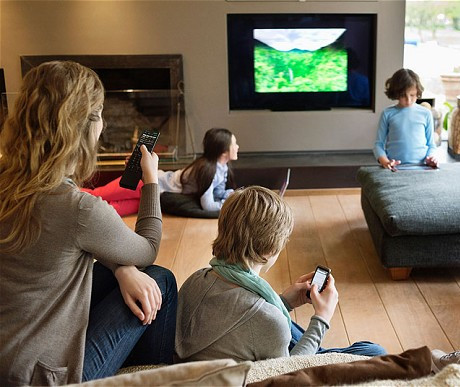
\includegraphics[height=3.4cm]{images/intro/currently.jpg}
				\caption{Les débuts de la Télévision face à son évolution}
			\end{figure}
		\end{frame}
	\begin{frame}{Problématique}
		\Large
		\begin{center}
		Quels sont les systèmes à mettre en œuvre pour offrir une expérience sociale depuis son poste de télévision ?
	\end{center}
	\end{frame}
	\begin{frame}
		\tableofcontents
	\end{frame}
	\section{La télévision interactive}
	\subsection{Influence des personnes}
	\begin{frame}{Influence des personnes}
\begin{itemize}
	\item Influence des téléspectateurs
		\begin{itemize}
			\item Sur le déroulement d'une émission en directe
			\item Sur le programme
			\item Sur la narration
		\end{itemize}
	\pause
		\vfill
	\item Communauté, réseaux sociaux
		\begin{itemize}
			\item Messages dans les bandeaux de l'émission
			\item Sur le site internet de l'émission
			\item \texttt{\#monEmission} sur Twitter
			\item Sur la page Facebook de la chaine/émission
		\end{itemize}
		\vfill
\end{itemize}
	\end{frame}
	\subsection{La communication}
	\begin{frame}{La communication}
\begin{itemize}
	\item Chat textuel
		\begin{itemize}
			\item Liste d'amis
			\item Éventuellement autre écran
		\end{itemize}
		\vfill
		\pause
	\item Chat vocal
		\begin{itemize}
			\item Difficile à utiliser \\
				$\Rightarrow$ Concentration\\
				$\Rightarrow$ Bruit de la TV
		\end{itemize}
		\vfill
\end{itemize}
	\end{frame}
	\subsection{Le partage}
	\begin{frame}{Le partage : aussi sociale que Facebook ?}
	\begin{itemize}
			\uncover<1->{
		\item Outils de communication
			\begin{itemize}
				\item Chat, message personnel, statut
			\end{itemize}
			\vfill
			}
			\uncover<2->{
		\item Jeux interactifs
			\begin{itemize}
				\item Score, partage du score, classement
			\end{itemize}
			\vfill
			\begin{figure}[H]
	\hspace{-20px}
				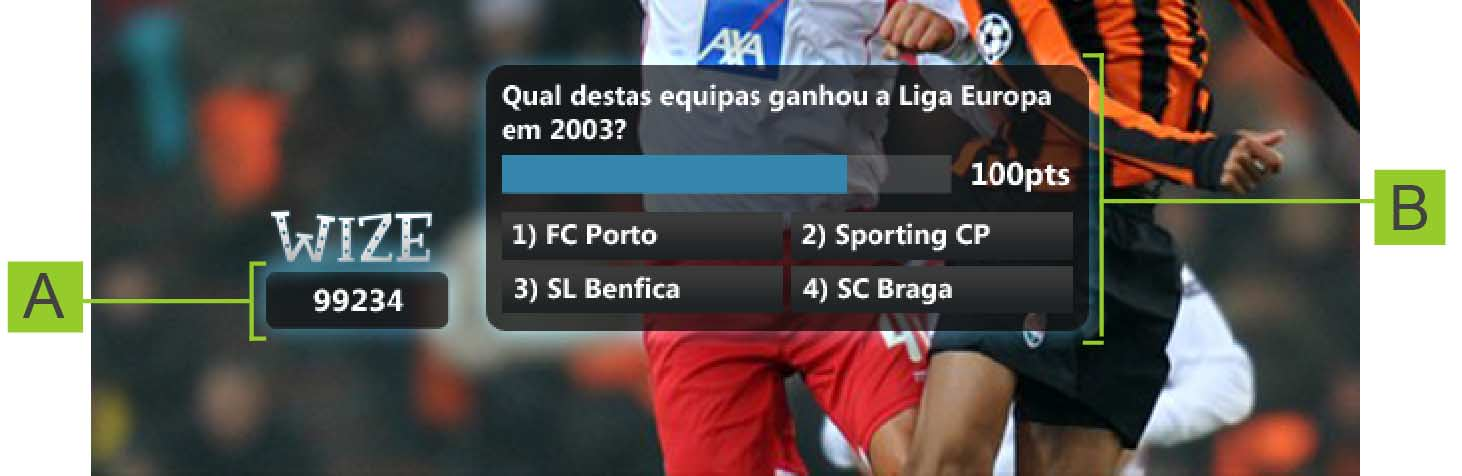
\includegraphics[height=3.0cm]{images/wize/1.png}
				\caption{Exemple du jeu interactif Wize\newline
				\scriptsize © \bsc{Almeida}, J. \bsc{Abreu}, A. \bsc{Pinho}, D. \bsc{Costa}\newline  \textit{Engaging Viewers through Social TV Games}.}
			\end{figure}
			}
			\uncover<3->{
		\item Proposition de contenu en fonction de différents critères
			\vfill
			}
	\end{itemize}
\end{frame}
	\section{La télévision sur multi-écrans}
	\subsection{Utilisation de la télévision multi-écrans}
	\begin{frame}{Utilisation de la télévision multi-écrans}
		\begin{exampleblock}{Avantages}
			\begin{itemize}
					\uncover<1->{
				\item Ne perturbe pas le visionnage sur la TV
					}
					\uncover<2->{
				\item Se prête bien au social
					}
					\uncover<3->{
				\item Distinction du côté social et du côté spectateur
					}
					\uncover<4->{
				\item Accès aux informations
					}
			\end{itemize}
		\end{exampleblock}
		\begin{alertblock}{Inconvénients}
			\begin{itemize}
					\uncover<1->{
				\item Attention requise
					}
					\uncover<2->{
				\item Désocialisation du monde réel
					}
					\uncover<3->{
				\item Créateur d'addiction
					}	
			\end{itemize}
		\end{alertblock}
	\end{frame}
	\subsection{Écrans externes}
	\begin{frame}{Écrans externes}
\begin{itemize}
	\item Répartition de contenu sur plusieurs écrans
		\begin{itemize}
			\item Télévision
			\item Smartphones et Tablettes
			\item Ordinateur
		\end{itemize}
\end{itemize}
	\end{frame}
	\section{Les systèmes et services TV}
	\subsection{Box et périphériques}
	\begin{frame}{Box et périphériques}
		\begin{itemize}
			\item Système $\rightarrow$ Services
		\pause
			\item Lien entre Box et autres périphériques
		\pause
			\item Périphériques externes
				\begin{itemize}
					\item Tablettes / Smartphones / PC
					\item Périphériques spécifiques
				\end{itemize}
		\end{itemize}
	\end{frame}
	\subsection{Cloud}
	\begin{frame}{Cloud}
		\begin{itemize}
			\item Synchronisation
		\pause
			\item Mise en place d'API
		\end{itemize}
		\begin{exampleblock}{Avantages}
			\begin{itemize}
				\item IHM identique sur chaque périphériques connectés
				\item Passage d'un écran à un autre sans << perte d'informations >>
				\item Poursuivre le visonnage hors de chez soi en se connectant au cloud
			\end{itemize}
		\end{exampleblock}
	\end{frame}

	\section*{Conclusion}
	\begin{frame}{Conclusion}
		\begin{itemize}
			\item TV $\rightarrow$ Sociale
				\pause
			\item Interactive
				\pause
			\item TV sur plusieurs écrans\ldots
				\pause
			\item \ldots et différents systèmes
		\end{itemize}
		\begin{figure}[H]
			\centering
			\vspace{-17px}
			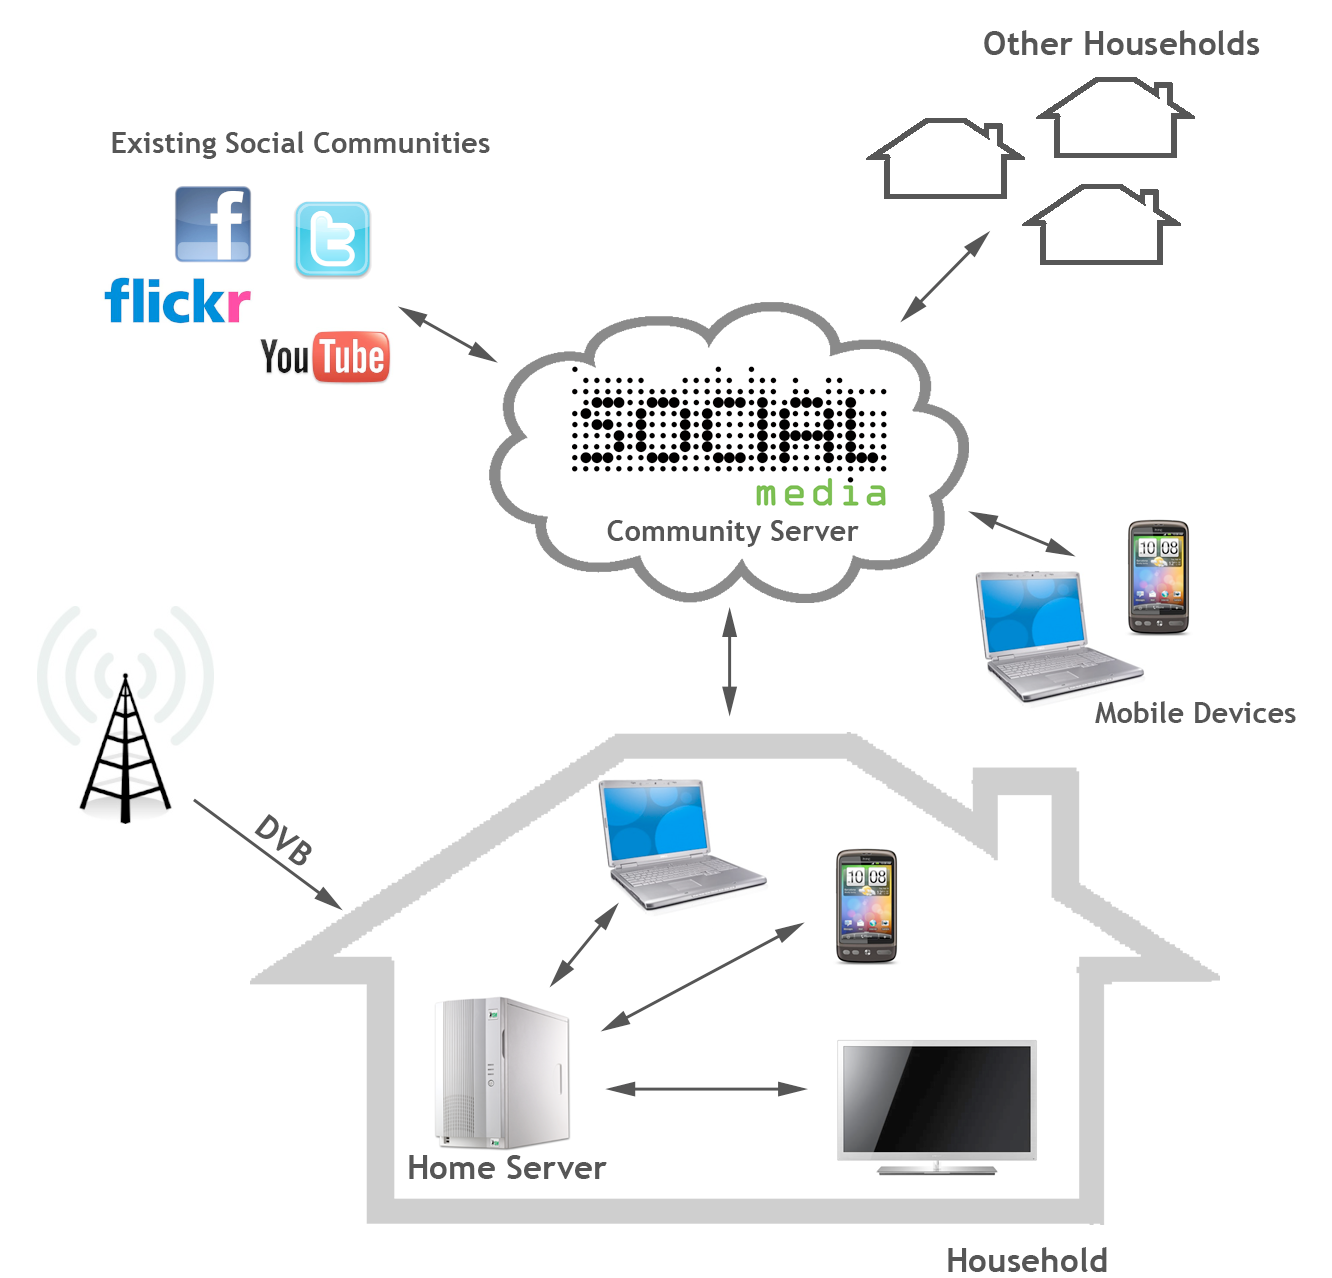
\includegraphics[width=5.4cm]{images/conclu.png}
			\scriptsize{
			\caption{SocialMediaFramework\newline 
			\tiny © Jan \bsc{Hess}, Benedikt \bsc{Ley}, Corinna \bsc{Ogonowski}, Lin \bsc{Wan}, Volker \bsc{Wulf}\newline
			\textit{Jumping between Devices and Services: Towards an Integrated Concept for Social TV}
			}
		}
		\end{figure}
	\end{frame}

	\begin{frame}{Avez-vous des questions ?}
		\begin{figure}[H]
			\centering
			
\includegraphics[width=5cm]{questions.png}
		\end{figure}
	\end{frame}

\end{document}
